\documentclass{article}

\usepackage{amsmath, amsthm, amssymb, amsfonts}
\usepackage{thmtools}
\usepackage{graphicx}
\usepackage{setspace}
\usepackage[a4paper, top=1in, bottom=1in, left=1in, right=1in]{geometry}
\usepackage{float}
\usepackage{hyperref}
\usepackage[utf8]{inputenc}
\usepackage[latvian]{babel}
\usepackage{framed}
\usepackage{microtype}
\usepackage[dvipsnames]{xcolor}
\usepackage{indentfirst}
\usepackage{tcolorbox}
\usepackage{fontspec}
\usepackage{makeidx}

\graphicspath{{img/}}
\setmainfont{DejaVu Serif}


\colorlet{LightGray}{White!90!Periwinkle}
\colorlet{LightOrange}{Orange!15}
\colorlet{LightGreen}{Green!15}

\newcommand{\HRule}[1]{\rule{\linewidth}{#1}}

\declaretheoremstyle[name=Theorem,]{thmsty}
\declaretheorem[style=thmsty,numberwithin=section]{theorem}
\tcolorboxenvironment{theorem}{colback=LightGray}

\declaretheoremstyle[name=Proposition,]{prosty}
\declaretheorem[style=prosty,numberlike=theorem]{proposition}
\tcolorboxenvironment{proposition}{colback=LightOrange}

\declaretheoremstyle[name=Principle,]{prcpsty}
\declaretheorem[style=prcpsty,numberlike=theorem]{principle}
\tcolorboxenvironment{principle}{colback=LightGreen}

\setstretch{1.2}
\geometry{
    textheight=9in,
    textwidth=5.5in,
    top=1in,
    headheight=12pt,
    headsep=25pt,
    footskip=30pt
}

\makeindex
% ------------------------------------------------------------------------------

\begin{document}

% ------------------------------------------------------------------------------
% Cover Page and ToC
% ------------------------------------------------------------------------------

\title{ \normalsize \textsc{}
		\\ [2.0cm]
		\HRule{1.5pt} \\
		\LARGE \textbf{\uppercase{Le Graph CHEATSHEET}
		\HRule{2.0pt} \\ [0.6cm] \LARGE{Yeah} \vspace*{10\baselineskip}}
		}
\date{}
\author{\textbf{Author} \\ 
		Graph LORD}

\maketitle
\newpage

\tableofcontents
\newpage

% ------------------------------------------------------------------------------

\section{Pamatjēdieni}
\textbf{Def.} Grafs G ir kopu pāris (V,E), kur V ir netukša kopa, kas sastāv no elementiem virsotnēm, un E ir kopa, kas sastāv no šķautnēm, kas savieno dažādu atsevišķu virsotņu pārus. Šī definīcija neiekļauj cilpas.\index{grafs!definīcija}

\textbf{Def.}  Ja u ∈ E (x1 , x2 ), tad saka, ka šķautne ved no virsotnes x1 uz virsotni x2 , bet trijnieku (x1 , u, x2 ) sauc par grafa incidenci. Ja u ir šķautne, kas ved no x1 uz x2 , tad saka, ka x1 un x2 indicē jeb pieder šķautnei.  Un otrādi - ka u indicē jeb pieder virsotnēm x1 un x2.\index{incidence}

\textbf{Def.}  Grafu sauc par galīgu, ja tam ir galīgs skaits šķautņu un virsotņu. Ja u indicē x1 un x2 , tad x1 un x2 ir gala virsotnes.\index{galīgs grafs}

\textbf{Def.} Neorientēta šķautne ved gan no x1 uz x2 , gan otrādi. Orientēta šķautne ved vienā virzienā, piem., no x1 uz x2. Ja šķautne, kas ved no x1 uz x2 ir orientēta, tad x1 sauc par sākuma, bet x2 par beigu virsotni. \index{orientēta šķautne}\index{neorientēta šķautne}

\textbf{Def.} Šķautni, kuras gala virsotnes sakrīt sauc par cilpu. Pretējā gadījumā to dažkārt sauc par īstu šķautni.\index{cilpa}

\section{Grafu klases}

\textbf{Def.}  Grafam vienmēr ir vismaz viena virsotne, bet tam var nebūt neviena šķautne. Grafu, kam nav šķautņu sauc par bezšķautņu grafu. Grafu, kam nav īstu šķautņu (tikai varbūt cilpas) sauc par triviālu grafu.\index{bezšķautņu grafs}\index{triviāls grafs}

\textbf{Def.} Grafu sauc par orientētu, ja tam nav šķautņu, kas nebūtu orientētas, un par neorientētu, ja tam nav šķautņu, kas nebūtu neorientētas.  Jaukts ir tāds grafs, kam ir gan orientētas, gan neorientētas šķautnes, neskaitot cilpas.\index{orientēts grafs}\index{neorientēts grafs}

\textbf{Def.} Ja ir dots patvaļīgs orientēts grafs G=(V,E) tad Ĕ (x, y ) = E (y , x) G apvērstais grafs - apvērš škautņu orientācijas. E (x, y ) = E (y , x) u Ĕ (x, y ) G piesaistītais grafs - atmet šķautņu orientācijas. \index{piesaistītais grafs}\index{apvērstais grafs}

\textbf{Def.} Grafu sauc par vienkāršu jeb unigrafu, ja no katras tā virsotnes uz katru citu ved ne vairāk kā viena šķautne. Pretējā gadījumā (ja ir paralēlas šķautnes) - to sauc par daudzkāršu jeb multigrafu.\index{unigrafs}\index{multigrafs}

\textbf{Def.} Par Berža grafu sauc ikvienu vienkāršu orientētu grafu, bet par parastu grafu - ikvienu neorientētu grafu bez cilpām.

\textbf{Def.} Patvaļīgā grafā virsotni y sauc par blakusvirsotni virsotnei x, ja no x ved šķautne uz y.
Līdzīgi divu vai vairāk dažādas šķautnes sauc par blakusšķautnēm, ja tām ir kopīga virsotne.

\textbf{Def.} Parastu grafu, kam jebkuras divas dažādas virsotnes ir blakusvirsotnes sauc par pilnu grafu. Katram fiksētam virsotņu skaitam tāds ir tikai viens. Pilnu grafu ar p virsotnēm parasti apzīmē ar Kp .

\textbf{Def.} Par zvaigznes grafu sauc parastu grafu, kurā ir tāda virsotne, kas ir. Vienīgā blakusvirsotne katrai no pārējām.  Šāds grafs katrai fiksētai virsotnei ir tikai viens. Zvaigznes grafu ar p virsotnēm parasti apzīmē ar Sp −1 (p-1 ir staru skaits).

\textbf{Def.}  Grafu sauc par vienkāršu jeb unigrafu, ja no katras tā virsotnes uz katru citu ved ne vairāk kā viena šķautne. Pretējā gadījumā (ja ir paralēlas šķautnes) - to sauc par daudzkāršu jeb multigrafu.  Par Berža grafu sauc ikvienu vienkāršu orientētu grafu, bet par parastu grafu - ikvienu neorientētu grafu bez cilpām.

\textbf{Def.}  Parastu grafu, kam jebkuras divas dažādas virsotnes ir blakusvirsotnes sauc par pilnu grafu (complete graph).  Katram fiksētam virsotņu skaitam tāds ir tikai viens Pilnu grafu ar n virsotnēm parasti apzīmē ar Kn
|E | =n C2

\textbf{Def.}  Grafs ir divdaļīgs (bipartite), ja tā virsotnes var sadalīt 2 kopās K un L tā, lai katrai šķautnei uv ∈ E viena no virsotnēm pieder K un otra L, t.i., u ∈ K , v ∈ L.  Pilnam divdaļu (complete bipartite) grafam ir visas iespējamās šķautnes starp abu virsotņu kopu K un L virsotnēm.  Pilnu grafu ar n virsotnēm parasti apzīmē ar Kn,m.  Divdaļu grafam raksturīgi, ka visi cilki ir ar pāra skaita garumu (taču var arī nebūt divdaļu grafā cikli).

\textbf{Def.}  Par zvaigznes (star) grafu sauc parastu grafu, kurā ir tāda virsotne, kas ir vienīgā blakusvirsotne katrai no pārējām.  Zvaigznes grafu ar p virsotnēm parasti apzīmē ar Sp −1 (p-1 ir staru skaits).

\textbf{Def.}  Par rata (wheel) grafu ar kārtu n sauc grafu kas sastāv no n-1 gara cikla, kura ikviena no virsotnēm ir savienota ar vienu kopīgu virsotni.  Rata grafu ar n virsotnēm parasti apzīmē ar Wn.

\subsection{Sakarīgs grafs}

\textbf{Def.}  Grafs ir sakarīgs, ja jebkurām virsotnēm u, v eksistē ceļš no u uz v.

\textbf{Def.}  Grafa sakarīgā komponente G'=(V',E'), kur V' ir maksimālā virsotņu kopa ar īpašību, ka katrām divām virsotnēm u,v ∈ V 0 eksistē ceļš u → v , E':uv ∈ E , u ∈ V 0 , v ∈ V 0 .  Virsotnes atvērta apkārtne NG (v ) = {u|uv ∈ E } - visas virsotnes, kas ir blakusvirsotnes v ∈ G.

\textbf{Def.} Virsotnes slēgta apkārtne NG [v ] = {u|uv ∈ E } u {v ∈ V } - visas virsotnes, kas ir
blakusvirsotnes v ∈ G un ietver arī pašu virsotni v.

\textbf{Def.}  Par brīvu sauc tādu virsotni, kurai pieder viena īsta šķautne. Par izolētu sauc tādu virsotni, kurai nepieder neviena īsta šķautne.  Ja virsotnei nav neviena šķautne, pat ne cilpa, tad to sauc par bezšķautņu virsotni.


\section{Grafa raksturlielumi}

\textbf{Def.}  Par neorientēta grafa virsotnes pakāpi dv (degv ) sauc skaitli, ko iegūst saskaitot šai virsotnei piederošo īsto šķautņu skaitu ar divkāršotu tai piederošo cilpu skaitu.  Vizuāli tas ir virsotnei piederošķautņu galu skaits, vienāds ar atvērtas apkārtnes virsotņu skaitu min pakāpe δ(G ) max pakāpe ∆(G )

\textbf{Def.} Par homogēnu (regulāru, r-regulāru) grafu sauc tādu grafu, kam visu virsotņu pakāpes ir vienādas.
degG v = δ(G ) = ∆(G ) = r ∀v ∈ V (G)

\textbf{Def.}  Par neorientēta grafa virsotnes pakāpi dv (degv ) sauc skaitli, ko iegūst saskaitot šai virsotnei piederošo īsto šķautņu skaitu ar divkāršotu tai piederošo cilpu skaitu. Vizuāli tas ir virsotnei piederošķautņu galu skaits.

Virsotnes pakāpe \textbf{T. }Virsotņu pakāpju summa = divkārš šķautņu skaits grafā.  degv = 2|E (G )| v ∈ V (G)

\textbf{S. } Grafā ir pāra skaits virsotņu ar nepāra pakāpēm.

P.  Katrā sakarīgā komponentē ir pāra skaits virsotņu ar nepāra pakāpi.

\textbf{S. } Ja grafā ir tieši 2 virsotnes ar nepāra pakāpi, tad eksistē ceļš no vienas uz
otru.

\section{Virsotņu virknes}

\textbf{Def.}  Par maršrutu (walk) grafā sauc tādu šī grafa virsotņu un šķautņu virkni x0 u1 x2 u2 x3 ...ul xl , kur l ≥ 0 un katrs trijnkieks (xi −1 , ui , xi ) ir grafa incidence.Tas ir, katra šķautne ui ved no virsotnes xi −1 uz xi .

\textbf{Def.}  Virsotni x0 sauc par maršruta sākuma virsotni un virsotni xl sauc par maršruta beigu virsotni, bet l sauc par maršruta garumu.  Maršrutu sauc par noslēgtu, ja tā beigu virsotne sakrīt ar sākuma virsotni (u0 = ul ).  0-maršruts sastāv no vienas virsotnes. Tas ir triviāls jeb tukšs marštuts.

\textbf{Def.}  Maršrutu sauc par ceļu/ķēdi (path), ja visas virsotnes ir dažādas.  Maršrutu sauc par cilku (cycle), ja noslēgtā maršrutā visas virsotnes ir dažādas.

\textbf{T.}  Ja ir maršruts a→ b, tad ir arī ceļš a → b.

\subsection{Divdaļīgs grafs}

\textbf{T.}  Grafs ir divdaļīgs ⇔ katram ciklam ir pāra garums

\subsection{Divdaļu grafa sakārtojuma konstruēšanas algoritms}
ievieto kādu virsotni u virsotņu kopā K (iekrāso vienā krāsā)
ievieto visas virsotnes v, kas ir incidentas u, virsotņu kopā L (iekrāso
otrā krāsā)
ieveto visas virsotnes v, kur īsākais ceļš no u uz v sastāv no 2, 4, ...  šķautnēm virsotņu kopā K (turpina krāsot iepriekšējā solī iekrāsoto virsotņu blakusvirsotnes pretējā krāsā)
ieveto visas virsotnes v, kur īsākais ceļš no u uz v sastāv no 3, 5, ...
šķautnēm virsotņu kopā L (turpina krāsot iepriekšējā solī iekrāsoto virsotņu blakusvirsotnes pretējā krāsā)


\section{Grafu izomorfisms}

\textbf{Def.}  Divi grafi G un G' ir izomorfi, ja pastāv savstarpēji viennozīmīgs attēlojums (bijekcija) starp grafa G un grafa G' virsotnēm, tāda ka virsotnes ir incidentas grafā G ⇔ ja atbilstošās virsotnes ir incidentas grafā G'.
Šādu savstarpēji viennozīmīgu atbilstību, kas saglabā virsotņu incidenci sauc par izomorfismu.  Izomorfos grafos ir: vienāds skaits virsotņu; vienāds skaits šķautņu; vienāds skaits virsotņu ar noteiktām virsotņu pakāpēm, turklāt; izomorfisms saglabā virsotņu pakāpes, tas ir, atbilstošajām virsotnēm; abos grafos ir vienāda pakāpe strukturālas līdzības (piem., divdaļīgs grafs, regulārs grafs).

Sistemātiska pārbaude, pārbaudot katru virsotni. Piem., sāk ar 5 un e (abām degv=1).

\subsection{Papildgrafs}

\textbf{Def.}  Par grafa G=(V , E ) papildgrafu Ḡ = (V , Ē ) sauc grafu, kurš satur visas grafa G virsotnes, bet šķautņu kopu veido tās virsotnes, kas G nav incidentas.  Grafa G apvienojums ar Ḡ veido pilnu grafu divi grafi G1 un G2 ir izomorfi ⇔ G¯1 un G¯2 ir izomorfi papildgrafu var izmantot grafu izomorfisma noteikšanā

\section{Planāri grafi}
Dabisks grafu piemērs ir ceļu kartes. Šādas kartes raksturo īpašība - tos var uzzīmēt ar šķautnēm (ceļiem) krustojoties tikai krustpunktos virsotnēs (krustcelēs).
\textbf{Def.}  Grafs ir planārs, ja to var uzzīmēt plaknē tā, ka šķautnes nekrustojas.  

\subsection{Apakšgrafs, parciālgrafs, daļgrafs}
\textbf{Def.}  Grafa G apakšgrafs G' ir grafs, ko veido grafa G virsotņu un šķautņu kopu apakškopas.  Par grafa G apakšgrafu sauc tādu grafu G', ko iegūst atmetot grafa G jebkuru skaitu virsotņu kopā ar tām piederošajām šķautnēm un tāpat, jebkuru skaitu šķautņu bez to gala virsotnēm
Izmetot šķautnes no planāra/plakana grafa → iegūst planāru/plakanu grafu pievienojot jaunas šķautnes planāram/plakanam grafam → var grafu padarīt neplanāru/neplakanu.

\textbf{Def.}  Maksimāli planārs grafs - ja tas pārstāj būt parasts un planārs pēc jaunas šķautnes pievienošanas vienalga starp kurām divām tā virsotnēm.

Jebkurš grafs ar n virsotnēm ir pilna grafa Kn apakšgrafs ja divi grafi ir izomorfi, tad apakšgrafi, kas veidojušies no atbilstošām virsotnēm un šķautnēm arī ir izomorfi apakšgrafu var izmantot grafu izomorfisma noteikšanā

\textbf{Def.} Par grafa G = (V,E) parciālgrafu sauc grafu G 0 = (V , E *), E* ⊂ E , kura virsotņu kopa ir vienāda ar grafa G virsotņu kopu, bet šķautņu kopa ir daļa no G šķautņu kopas.  Grafa G = (V,E) daļgrafs G 0 = (V 0 , E 0 ) satur gan daļu no grafa virsotnēm, gan šķautnēm, tomēr katrai šķautnei e ∈ E 0 virsotnes e = (vi , vj ) pieder kopai V 0 ⊂ V .

\textbf{Def.} Plakans grafs ir tāds planārs grafs, kas ir uzzīmēts tā, ka šķautnes nekrustojas.  Plakans grafs sadala plakni regionos.
\textbf{Def.}  Cilku, kas ierobežo plaknes daļu, kura nesatur ne virsotnes, ne šķautnes sauc par robežcilku.
\textbf{Def.} Par plakana grafa skaldni (face) sauc ikvienu plaknes daļu (arī neierobežoto, bezgalīgo), ko norobežo robežcikls.  Ja grafā ciklu nav - par skaldni uzskata visu planki.  Ārējo robežciklu veido šķautnes, kas atdala grafu no bezgalīgās skaldnes.  Skaldņu skaitu apzīmē ar r. Ja skatās uz jebkuru skaldni maksimālā planārā grafā - visi ir trīsstūri jebkuras skaldnes robeža var tikt pārveidota kā ārējā robeža. Skaldņu skaits paliek nemainīgs.  Skaldnes pakāpe df ir šķautņu skaits, kas ierobežo skaldni.

\subsection{Apļa-hordu metode (Circle-chord method)}
→ no pretējā
pieņem, ka ir plakans/planārs
ja pretruna - tad pieņēmums ir aplams
Atrod cilku, kas satur visas grafa virsotnes (var gadīties, ka nav tāds cikls, bet šobrīd skatamies gadījumus, kas ir) uzzīmē ciklu kā lielu apli atlikušās šķautnes-hordas jāzīmē iekšpus vai ārpus apļa plaknē pirmo hordu izvēlas zīmēt, piemēram, ārpus apļa.
Šī horda liks citām būt iezīmētām iekšpusē (ja zīmētu ārpusē, tad krustotos) Iekšpuses hordas savukārt liks citas zīmēt ārpusē.  Ja nonāk pie situācijas, kad nav iespēja ievilkt šķautni bez krustošanās, tad nav planārs.
Ja var visas šķautnes savilkt bez krustošanās, tad ir plakans.  Nav nozīme, vai pirmo šķautni velk iekšpus vai ārpus apļa.  Pastāv efektīvi algoritmi, kā noteikt, vai grafs ir planārs, atšķirībā no izomorfisma.

\subsection{Sakarīga komponente}
\textbf{Def.}  Par grafa G sakarīgo komponenti jeb komponenti sauc jebkuru maksimālu sakarīgu apakšgrafu.
Maksimāls nozīmē, ka apakšgrafam zūd sakarības īpašība, ja tam pievieno vēl kādu no grafa G virsotnēm. Tas nozīmē, ja apakšgrafu var papildināt līdz lielākam, bet tomēr vēl sakarīgam, tad vēl nav bijusi aplūkota komponente.  Sakarīgu komponenšu skaitu apzīmē ar s.  Grafu G sauc apr viensakarīgu, ja tas ir sakarīgs, bet atmetot vienu virsotni v līdz ar tai incidentām šķautnēm, rodas nesakarīgs grafs. Šādu virsotni v sauc par sasaistes virsotni.
Grafu G sauc par divaskarīgu, ja tas nav viensakarīgs, bet atmetot 2 virsotnes vi un vj un tām incidentās šķautnes - rodas nesakarīgs grafs. Trīssakarīgs ir tāds grafs, kas nav divsakarīgs, bet atmetot 3 virsotnes ar tām incidentām šķautnēm, rodas nesakarīgs grafs.

\subsection{Eilera teorēma}

\textbf{T.} Eilera teorēma par plakaniem grafiem - Ja G ir sakarīgs un plakans grafs ar p virsotnēm, q šķautnēm un r skaldnēm, tad p − q + r = 2.
p - virsotņu skaits, q - šķautņu skaits, r - skaldņu skaits
\textbf{S. } Jebkurā sakarīgā plakanā grafā izpildās p − q + r − s = 1.  p - virsotņu skaits, q - šķautņu skaits, r - skaldņu skaits, s - sakarīgo komponenšu skaits

\textbf{T.}  Ja G ir maksimāls plakans grafs ar p ≥ 3 virsotnēm un m šķautnēm, tad q = 3p − 6.  p - virsotņu skaits, q - šķautņu skaits
\textbf{S. } Ja grafs G ir sakarīgs plakans grafs ar p ≥ 3 virsotnēm un q šķautnēm, tad q ≤ 3p − 6.  p - virsotņu skaits, q - šķautņu skaits

Tomēr arī neplanāri grafi var apmierināt šīs sakarības.  Ja neizpildās ⇒ nav plakans; Ja izpildās ⇒ vēl nevar droši secināt, ka ir plakans. L.  Ja G ir plakans sakarīgs grafs ar p virsotnēm un q šķautnēm un bez trīsstūru skaldnēm, tad q ≤ 2p − 4

\subsection{Planāru grafu atpazīšana}

Kā atpazīt neplanārus grafus?
Šie 3 apgalvojumi ir ekvivalenti:
Grafs ir planārs
Grafs nesatur K5 vai K33 kā konfigurāciju
Grafs nesatur K5 vai K33 kā minoru

Teiksim, ka grafs G ir reducējams uz grafu G', ja tas sakrīt ar G' vai arī G' var iegūt no G veicot vienu vai vairākas reizes patvaļīgā secībā šādas redukcijas procedūras: no grafa izmet vienu (jebkuru) šķautni, atstājot galavirsotnes no grafa izmet jebkuru virsotni un tai incidentās škautnes ja x u y v z ir divu šķautņu ceļš grafā un virsotnei y ir pakāpe 2, bet x = 6 z, tad abas šķautnes u un v un to kopīgo virsotni izņem, bet vietā ielik jaunu šķautni ar gala virsotnēm x un z.  Piezīme. Izmantojot pirmos divus punktus, jebkuru grafu var reducēt uz vienu virsotni.

\subsection{Kuratovska un Pontrjagina teorēma}

\textbf{T.}  Grafs nav planārs ⇔ to var reducēt uz K5 vai K33 Iepriekš esam pierādījuši, ka K5 vai K33 nav planāri.  Redukcijas ceļā neplanāru grafu var iegūt tikai no neplanāra grafa.
\textbf{S. } Grafs ir planārs ⇔ ja to nevar reducēt ne uz K5 , ne K33

\textbf{Kuratovska T.} Grafs G ir planārs ⇔ ja tas neveido ne K5 , ne K33 daļgrafu, nedz arī tiem līdzīgus (homomorfus) grafus

\textbf{Def.}  Plakanam grafam var piekārtot duālo grafu, kurā skaldnes=virsotnes un robežškautnes=šķautnes (t.i., šķautnes saglabājas).

\subsection{Konfigurācija}
\textbf{Def.} Grafu ir iespējams pārveidot, pievienojot virsotnes šķautņu vidū.  Rezultātā tiek iegūts grafs, kas vairs nav, piem., K33 , un neietver K33 kā apakšgrafu, tomēr tas joprojām ir neplanārs.  Pievienojot neplanāram grafam virsotnes nevar iegūt planāru grafu.

\textbf{Def.}  Elementāra konfigurācija tiek iegūta grafam G noņemot šķautni e=uv un pievienojot jaunu virsotni w un divas šķautnes uw un vw.  Grafa konfigurācija ir grafs, kas iegūts no G secīgi veicot 0 vai vairākas elementāras konfigurācijas.

\subsubsection{K33 konfigurācija}
\textbf{T.}  Jebkura grafa G konfigurācija H ir planāra ⇔ G ir planārs (Šķautņu sadalīšana nemaina planaritāti.)

\textbf{Def.}  Saka, ka grafs ir K33 konfigurācija, ja tas var tikt iegūts no K33 ,
pievienojot virsotnes šķautņu vidū.

\textbf{Def.}  Saka, ka grafs iir K5 konfigurācija, ja tas var tikt iegūts no K5 , pievienojot
virsotnes šķautņu vidū.

K5 pievienotas virsotnes ar šķautnēm. K5 ir izveidotā grafa apakšgrafs. K5 šķautnes sadalītas ar jaunām virsotnēm. K5 nav apakšgrafs, bet nav arī planārs. Ja izņemtu jaunas virsotnes, tad arī nav planārs.

\textbf{Kuratovska T.} Grafs G ir planārs ⇔ ja tas nesatur K5 vai K33 konfigurāciju

\subsection{Grafu defucēšana}

Škautņu savilkšana:
1 šķautņu dzēšana G \ e
2 šķautņu savilkšana - abas šķautnes galavirsotnes savelk kopā (šķautnes e gala virsotnes u un v izņem un aizvieto ar w, w ir incidenta ar visām u un v blakusvirsotnēm) (multigrafs, parasts grafs)

\textbf{Def.}  Grafs H ir grafa G minors, ja to var iegūt no G veicot šādas redukcijas: dzēš šķautni savelk šķautni dzēš izolētas virsotnes (Grafs G ir pats sev minors, pielietojot 0 redukcijas)

\subsection{Vāgnera teorēma}

Vāgnera teorēma (Wagner's theorem) - Katrs grafs, kas ir izomorfs G minoram, arī ir G minors.
\textbf{Def.}  Grafs G satur grafu H kā minoru, ja G satur apakšgrafu G', ko var savilkt uz H.
Vāgnera \textbf{T. } Grafs G ir planārs ⇔ tam nav K5 vai K33 minora (G nesatur K5 vai K33 kā minoru)

Kuratovska \textbf{T. }vs Vāgnera \textbf{T. }Kāda saistība starp abām teorēmām? G minoru ne vienmēr var pārveidot G konfigurācijā. Ja G satur ≥ 1 K5 vai K33 kā minoru, tad tas satur ≥ 1 K5 vai K33 kā konfigurāciju.

\section{Grafu krāsošana}

\textbf{Def.}  Pareizi nokrāsots grafs - piešķirt grafa virsotnēm krāsas tā, lai incidentām virsotnēm būtu atšķirīgas krāsas.  Hromatiskais skaitlis χ ir mazākais skaits krāsu, ar ko var pareizi nokrāsot grafu.  k-krāsojums - grafs G ir nokrāsots k krāsās. Ja ir nokrāsots ⇒ grafs G ir k-nokrāsojams, χ = k, grafs G ir k-hromatisks.

\textbf{Def.}  Dots grafs G = (V , E ) K-krāsojums sadala virsotņu kopu V k kopās V1 , V2 , ...Vk , kur katra kopa Vi ir neatkarīgu virsotņu kopa (neviena no virsotnēm nav savā starpā incidentas).  V = V1 u V2 u ... u Vk Vi ∩ Vj = ∅ visiem i 6= j
Neatkarīgās kopas V1 , V2 , ...Vk sauc par krāsu klasēm.

Ar cik krāsām var nokrāsot dotu grafu?  Grafam ar ≤ 15 virsotnēm parasti nav grūti atrast hromatisko skaitli.  Lai pārbaudītu, ka grafa hromatiskias skaitlis ir k, ir jāpārbauda arī, ka grafs nevar tikt nokrāsots k − 1 krāsās.  Mērķis parādīt, ka jebkurš k − 1 krāsojums noved pie tā, ka divas incidentas virsotnes ir vienā krāsā.
 
\subsection{Daži fakti}
Ja G ir n virsotnes,;
tad χ(G ) ≤ n;
χ(G ) = 1 ⇔ G ir tukšs grafs;
χ(Kn ) = n ⇒ G ir pilns grafs;
Cikls ar pāra šķautnēm χ(C2n ) = 2;
Cikls ar nepāra šķautnēm χ(C2n=1) = 3;
Rats ar pāra zariem χ = 3;
Rats ar nepāra zariem χ = 4;
Ja H ir apakšgrafs χ(G ) ≥ χ(H).

\subsection{2-hromatiski grafi}
Fakts: Katrs grafs-koks ar vismaz 2 virsotnēm ir 2-hromatisks.
\textbf{T. }Grafa G hromatiskais skaitlis χ(G ) ir 2 ⇔ G ir divdaļīgs.
\textbf{T. }Grafa G hromatiskais skaitlis χ(G ) ir 2 ⇔ G ir divdaļīgs.
 
\subsection{Hromatiskā skaitļa augšājā robeza}
\textbf{T. } Katru grafu var nokrāsot ar d + 1 krāsām, kur d ir grafa maksimālā pakāpe, χ(G ) ≤ 4(G ) + 1.

\subsection{Planāru grafu krāsojums - Eilera formula}

Planārā grafā q ≤ 3p − 6, p ≥ 3, q - šķautņu sk., p - virsotņu sk.
\textbf{S. }(min pakāpe planārā grafā). Planārā grafā ir virsotne v, kam dv ≤ 5.
6 krāsu \textbf{T. }Jebkuru planāru grafu var pareizi nokrāsot ar 6 krāsām.
5 krāsu \textbf{T. }Ja grafs ir planārs, sakarīgs un vienkāršs, tad χ(G ) ≤ 5.

\section{Eilera ķēdes un cikli}

\textbf{Def.} Ķēde - maršruts, kurā nav šķautnes, kas atkārtotos
noslēgts maršruts - sākuma un beigu virsotnes sakrīt (x0 = xl )
cikls - noslēgta, netukša ķēde
elementāra/vienkārša ķēde - nav virsotnes, kas atkārtojas, izņemot
varbūt gala un sākuma virsotni

\textbf{Def.}  Eilera ķēde grafā ir jebkurš maršruts, kas satur visas grafa šķautnes.
Ja tāds maršruts ir cikls, tad to sauc par Eilera ciklu. (Satur katru grafa šķautni tieši 1 reizi) Grafu, kurā eksistē vismaz viens Eilera cikls sauc par Eilera grafu.
\textbf{T. } Ja grafā ir virsotne v ar nepāra pakāpi dv , tad tajā nav noslēgta Eilera maršruta (Eilera cikla).

\subsection{Eilera cikls. Algoritms.}
\textbf{Kā grafā konstruēt Eilera ciklu?}

Algoritms 1:
\begin{itemize}
	\item Veido maršrutu no brīvi izvēlētas virsotnes katrā solī ejot pa šķautni, pa kuru iepriekš nav iets, līdz tas vairs nav iespējam
	\item (Veidojas maršruts M0 )
	\item Aplūko grafu, kas sastāv no atlikušajām šķautnēm. (Komponentes G1 , G2 utt.)
	\item Katrai komponentei izveijo Eilera maršrutu (G1 → M1 , G2 → M2 utt.)
	\item Ievieto M1 , M2 utt. maršrutā M0
	\item Algoritms vienmēr atrod noslēgtu Eilera maršrutu (Eilera ciklu), ja tāds eksistē.
\end{itemize}
	
Veido maršruru katrā solī ejot pa šķautni, pa kuru nav iets. Veidojas maršruts M0 .
M0 : c → d → e → f → g → m → l → k → j → c Aplūko grafu, kas sastāv no atlikušajām šķautnēm. Komponentes G1 , G2 .  Katrai komponentei izveido Eilera maršrutu (G1 → M1 , G2 → M2 ).  Ievieto M1 , M2 maršrutā M0 .  M0 : c → d → ...M1 ... → d → e → f → g → ...M2 ... → g → m → l → k → j → c

[TK]

\subsection{Eilera grafs}

\textbf{T. } Grafs bez izolētām virsotnēm ir Eilera grafs ⇔ šis grafs ir sakarīgs un katrai tā virsotnei ir pāra pakāpe.
\textbf{T. } Ja grafā ir nenoslēgts Eilera maršruts, tad visām virsotnēm, izņemot sākuma un beigu, pakāpe dv ir pāra.
\textbf{T. } Grafā eksistē nenoslēgta Eilera ķēde ⇔ grafs ir sakarīgs un ar ≤ 2 virsotnēm ar nepāra pakāpi.

\subsubsection{Grafa sadalīšana}

Grafu sadala tā, ka katrā izdalītajā apakšgrafā ir atšķirīgas šķautnes Aplūko grafu G Var atrast divus 3 šķautņu ciklus Nav noteikti jābūt cikliem vai vienādām daļām
F = F1 , F2 , E (F1 ) u E (F2 ) = E (G )

\textbf{Def.}  Grafa sadalījums ir saime F ar apakšgrafiem F1 , F2 ...Fn , kas sastāv no atšķirīgām šķautnēm tā, ka uE (F ) = E (G ).  Ja katrs apakšgrafs saimē F ir cikls, tad sadalījumu sauc par cilku sadalījumu. Ja katrs apakšgrafs saimē F ir ceļš, tad sadalījumu sauc par ceļu sadalījumu.  nevar sadalīt ciklos, bet var izveidot ceļu sadalījumu viena šķautne-triviāls ceļš
\textbf{Def.}  Pāra grafs - visām virsotnēm ir pāra pakāpe
\textbf{T. } Grafa G šķautnes var sadalīt cikla sadalījumā ⇔ grafs G ir pāra grafs
\textbf{T. } Eilera grafs ⇔ pāra grafs ⇔ cilku sadalījums

\section{Hamiltona grafs}

\textbf{Def.}  Hamiltona ceļš ir ceļš, kas satur visas grafa virsotnes.  Hamiltona cikls ir cikls, kas satur katru grafa virsotni tieši vienu reizi.  Ja grafs satur Hamiltona ciklu, tad tas ir Hamiltona grafs.  Hamiltona cikls var nebūt Eilera cikls un otrādi.  Līdz šim nav atrasti pietiekamie un nepieciešamie nosacījumi tā eksistencei Daudzi grafu teorijas jautājumi pierādāmi grafos ar Hamiltona ciklu Hamiltona cikla noteikšanu var veikt ar pārlasi

\subsection{Hamiltona cikla noteikšana}
Kā grafā konstruēt Hamiltona ciklu? Izmanto līdzīgu spriešanu kā nosakot izomorfismu vai planaritāti fokusējas, lai noteiktu, ka grafā neeksistē Hamiltona cikls lai pierādītu - konstruē grafā potenciālu Hamiltona ciklu, līdz nonāk līdz pretrunai

\textbf{Likumi, kam jāizpildās, konstruējot Hamiltona ciklu:}
\begin{itemize}
	\item Pieņem, ka grafā ir Hamiltona cikls. Šādam ciklam jābūt tieši 2 šķautnēm incidentām katrai virsotnei. No tā seko:
	\item Ja grafā ir virsotnes ar pakāpi 2, tad abas šķautnes pieder Hamiltona ciklam
	\item Neveido apakšciklu, tas ir, ciklu, kas nesatur visas virsotnes
	\item Tā kā katrai virsotnei var būt tikai 2 šķautnes, tad pārējās (tās, kas nav izmantotas, lai konstruētu Hamiltona ciklu) jānoņem
\end{itemize}
	
\subsection{Kā grafā konstruēt Hamiltona ciklu?}
Likumi, kam jāizpildās, konstruējot Hamiltona ciklu
\begin{itemize}
	\item Ja grafā nav virsotne ar pakāpi 2, tad mēginājumu ceļā meklē Hamiltona ciklu.
	\item Kā sākuma virsotni izvēlas tādu, lai pē iespējas vairāk šķautnes pazustu var būt jāaplūko vairāki gadījumi ņem vērā simetriju, ja var piemērot
\end{itemize}
	
\subsection{Teorēmas}

\textbf{T. }Dīraka teorēma. Ja grafā no katras virsotnes iziet n/2 škaunes ≥ tajā ir Hamiltona ceļš.

\textbf{T. }Grīnberga teorēma.  (Var tikt izmantota, lai pierādītu, ka daži planāri grafi nesatur Hamiltona ciklu) Pieņem, ka planāram grafam G ir Hamiltona cikls. Grafu G uzzīmē jebkurā plakanā izkārtojumā.  ri - skaldņu skaits Hamiltona ciklā, ko ierobežo i šķautnes.  ri0 - skaldņu skaits ārpus Hamiltona cikla, ko ierobežo i šķautnes. 
Tad izpildās: (i − 2)(ri − ri0 ) = 0

\subsection{Turnīrs}
\textbf{Def.}  Turnīrs ir orientēts grafs, kurā starp katrām 2 virsotnēm ir tieši viena šķautne. Pilns grafs ar n virsotnēm Kn katra šķautne orientēta vienā virzienā virsotnes - komandas, šķautne uv - v uzvar u katrā šādā grafā ir orientēts ceļš (v1 v2 )...(vn−1 vn ), kas ietver visas virsotnes.

\textbf{T. } Katrā turnīrā ir Hamiltona ceļš.

\section{Koki}

\subsection{Definīcijas}

\textbf{Def.}  Koks ir sakarīgs grafs bez cilkiem

Standarta veids, kā zīmēt koku ar sakni, ir novietojot sakni augšā un atbilstoši tālāk virsotnes kārtot pa līmeņiem Sakne ir 0. līmenis No saknes uz katru koka virsotni ved unikāls ceļš Virsotnes x līmenis kokā norāda unikālā ceļa garumu no saknes a.  Ja grafs ir neorientēts, tad jebkura tā virsotne var būt sakne; orientētam grafam ir noteikta sakne.

\textbf{Def.}  Lapa - virsotne kokā ar pakāpi 1.  Mežš - grafs bez cikliem, ne obligāti sakarīgs (komponentes ir koki).

\textbf{Def.}  Ja p ir i līmeņa virsotne, c ir i + 1 līmeņa virsotne un pc ir šķautne, tad c ir p bērns; p ir c vecāks.  Ja ir virsotņu virkne v0 = p1 , v1 , ..., vk = d, kur v1 ir v0 bērns, v2 ir v1 bērns, ..., vk ir vk −1 bērns, tad d ir p pēctecis.

\textbf{Def.}  Šādi apgalvojumi ir ekvivalenti: (A) T ir koks; (B) T starp katrām 2 virsotnēm ir tieši viens ceļš; (C) T ir sakarīgs grafs, no kura izmetot jebkuru šķautni, T kļūst nesakarīgs Pierādījums (A ⇔ B)


\textbf{Def.}  Lapas ir koka virsotnes ar pakāpi 1, tās ir virsotnes bez bērniem.  Virsotnes ar bērniem ir iekšējās virsotnes.  Ja katrai iekšējai virsotnei ir 2 bērni, tad tas ir binārs koks.  Ja katrai iekšējai virsotnei ir m bērni, tad tas ir m-ārs koks.

\textbf{Def.}  Koka (ar sakni) augstums ir garākais ceļš no saknes vai ekvivalenti jebkuras virsotnes augstākais/lielākais līmenis.  Koks (ar sakni) ir līdzsvarā, ja visas lapas ir līmenī h un h-1. (Tie ir labi koki) M-āra koka līdzsvarošana minimizē tā augstumu.

\subsection{Teorēmas}

\textbf{T. } T ir koks ⇔ T ir grafs bez cikliem, kurā pievienojot šķautni starp jebkurām divām
nesavienotām virsotnēm rodas cikls

\textbf{S. } Katrā kokā ir ≥ 2 lapas, n ≥ 2.

\textbf{T. } Kokā ar n virsotnēm ir n-1 šķautne.

\textbf{T. } Mežā ar n virsotnēm un k komponentēm ir n-k šķautnes.

\textbf{T. } T ir koks ⇔ T ir sakarīgs grafs ar n virsotnēm un n-1 šķautnēm.

\textbf{T. } Ja T ir m-ārs koks ar n virsotnēm, no kurām i ir iekšējās virsotnes, tad n = mi + 1.

\textbf{S. } Ja T ir m-ārs koks ar n virsotnēm, i iekšējām virsotnēm un l lapām, tad zinot vienu no vērtībām (i, n vai l) abas pārējās attiecīgi var aprēķināt:
i : l = (m − 1)i + 1, n = mi + 1
l : i = (l − 1)/(m − 1), n = (ml − 1)/(m − 1)
n : i = (n − 1)/m, l = [(m − 1)n + 1]/m


%fix
\textbf{T. } Ja T ir m-ārs koks ar augstumu h un l lapām, tad: a) l ≤ mh un ja visas lapas ir augstumā h, l = mh; b) h ≥ dlogm le un ja koks ir līdzsvarā, h = dlogm le dr e noapaļo r uz nākošo lielāko veselo skaitli
\textbf{T. } Kokā ar n virsotnēm ir n-1 šķautne.
\textbf{S. } Katrā kokā ir ≥ 2 lapas, n ≥ 2.

\subsection{Prūfera virkne}

Koka virsotnes numurē. Katram kokam ar n numuriem izveido virkni a1 , a2 , ...an−2 ar garumu n − 2 sekojoša veidā: izvēlas l1 lapu ar mazāko numuru un ar a1 apzīmē blakusvirsotni; izdzēš l1 no koka un atkārto iepriekšējo punktu; apstājas, kad atlikušais koks ir reducēts uz 2 lapām, kas savienotas ar šķautni izveidojas virkne. \textbf{To }sauc par Prufera kodu/virkni (Prüfer sequence).  Tālāk var parādīt, ka katra šāda (n − 2) garuma virkne no n numuriem definē unikālu n numurētu koku: apvērš procedūru: var novērot, ka lapas (virsotnes ar pakāpi 1) nekad neparādās virknē pirmais numurs virknē ir kaimiņš lapai ar mazāko numuru mazākā numura lapa ir mazākais numurs, kas neparādās virknē, aplūkojot visu virsotņu numuru sarakstu atbilstoši ievieto tabulā li un tālāk vairs neaplūko atkārto procedūru palikušajām (n − 1) virsotnēm numurētajā kokā atbilstoši palikušajai (n − 3) virknei utt.

%[Insert example]

Apgalvojums
Katra virsotne ar pakāpi ≥ 2 parādās virknē a1 , a2 , ...an−2 .;  Kopā tiek nodzēstas n-2 no n-1 šķautnēm; Tiek nodzēsta ≥ 1 šķautne, kas ietver virsotni v; kad tiek nodzēsta pirmā no šķautnēm, v nav lapa; u ir lapa, li = u, ai = v



\subsection{Pārklājošais koks}

Koki piedāvā ietvaru problēmu risināšanā, kas ietver dažādu variantu secīgu aplūkošanu/izskatīšanu/izvēlēšanos
Daudzu no iepriekš aplūkotām problēmām (izomorfisms, Hamiltona cikls, hromatiskais skaitlis u.c.) datorizētā risināšana balstās uz kokiem.


\textbf{Def.}  Grafa G pārklājošais koks T (spanning tree) ir koks , kura visas šķautnes ir arī G šķautnes un tas ietver visas G virsotnes.

\subsection{Dažāda veida meklēšanas algoritmi}

\subsubsection{Meklēšana dziļumā (Depth-first spanning tree DFS)}

Algoritms
Izvēlas kādu virsotni par sakni un sāk veidot ceļu no saknes, kas sastāv no grafa šķautnēm ‘
katrā solī mēgina turpināt konstruēt koku no tekošās virsotnes
ceļš tiek turpināts, kamēr to nevar turpināt neatkārtojot jau kokā esošu virsotni
virsotne, kur šis ceļš apstājas, ir lapa
ja nav iespējams turpināt ceļu, tad atkāpjas uz iepriekšējo virsotni, t.i., dodas atpakaļ uz vecāka virsotni y šai lapai un cenšas turpināt ceļu citā virzienā
kad visi iespējamie ceļi no šī vecāka y un tā citiem bērniem ir izveidoti, tad kāpjas atpakaļ uz konkrētā vecāka y vecāka virsotni utt. līdz nonāk atpakaļ līdz saknei un ir pārbaudīti visi iespējamie ceļi no saknes

\subsubsection{Meklēšana plašumā (Breadth-first spanning tree BFS)}

Algoritms
Izvēlas kādu virsotni kā sakni, kas ir 0-līmenis un novieto visas izejošās šķautnes 1-līmenī kokā. Sekojoši nākošajā līmenī pievieno šķautnes, kas ir incidentas saknes blakusvirsotnēm, ja vien nav savienota ar kokā jau izmantotu virsotni, utt.

\subsection{Sakarīgo grafu pārklājošie koki}

Ja grafs nav sakarīgs, tad tam neeksistē pārklājošs koks.  Ja r ir sakne un u ir patvaļīga virsotne, tad ceļš ru, kas ir meklēšanas
plašumā kokā \textbf{T, }ir īsākais ceļš no r uz u sākotnējā grafā.
Īsākais ceļš: ru1 , u1 u2 , ..., uk −1 u
u1 - 1līmenis
u2 − ≤ 2 līmenis
...
uk −1 ≤ k-1 līmenis
u ≤ k līmenis


\subsection{Pārklājošā koka pielietojumi}

Vai grafs ir sakarīgs? Sākot ar virsotni r (sakni), konstruē pārklājošo koku T (ar DFS vai BFS) ja virsotņu skaits T = virsotņu skaitu G, tad G ir sakarīgs (citādi nē).

Grafa G sadalīšana sakarīgās komponentēs. Kamēr visas virsotnes nav ieliktas kādā komponentē: r - virsotne, kas nav nevienā komponentē K veido koku ar BFS K' - komponente, kas sastāv no visām v ∈ T un uv , u, v ∈ T .

Vai grafā ir cikls?  Katrai komponentei Ki uzkonstruē pārklājošo koku Ti. Ja ir šķautne uv, u, v ∈ Ki , uv ∈ / Ti, tad ir cikls.

Vai grafs ir divdaļīgs?  Konstruē pārklājošo koku T ar BFS.
r ∈ K ⇒ 1.līm. ∈ L ⇒ 2.līm. ∈ K ⇒ 3.līm. ∈ L...
K = r u (2.līm.) u (4.līm) u ...
L = (1.līm.) u (3.līm) u ...
Pārbauda, vai šķautnes uv, u ∈ K , v ∈ L

Neorientētu grafu var raksturot ar kaimiņmatricu, kas satur |V | = n rindas un kolonnas.  Katrai rindai un kolonnai atbilst viena virsotne.  Rindu un kolonnu secība ir vienāda.  Neorientētam grafam ai j = 1, ja virsotnes vi un vj ir kaimiņvirsotnes, t.i., tās abas in incidentas šķautnei e = [vi , vj ], pretējā gadījumā ai j = 0.  Sakarīguma pārbaude ar kaimiņmatricu.

\subsection{Minimālais pārklājošais koks (Minimal Spanning Tree (MST))}

\subsubsection{Definīcija}

Dots grafs, kurā šķautnēm ir garumi. Uzdevums atrast pārklājošo koku ar minimālo garumu (tiek summēts šķautņu garums).  Tā ir sarežgītāka problēma nekā atrast īsāko ceļu tīklā. Aplūkosim 2 algoritmus: Prima algoritmu un Kruskal algoritmu

\textbf{Def.} Minimālais aptverošais koks (MST) vai minimālā svara aptverošais koks ir savienota, ar malām svērta nevirzīta grafika malu apakškopa, kas savieno visas virsotnes kopā, bez cikliem un ar minimālo iespējamo kopējo malas svaru.

\subsubsection{Prima algoritms}
n - virsotņu skaits tīklā

Atkārtot sekojošo soli, kamēr kokā T ir n-1 šķautnes: pievieno T īsāko šķautni, starp virsotni, kas ir kokā T un virsotni, kas nav T (sākotnēji izvēlas jebkuru šķautni ar īsāko garumu).

\subsubsection{Kruskal algoritms}

Atkārtot sekojošo soli, kamēr kopā T ir n-1 šķautnes (sākumā kopa T ir tukša): pievieno T īsāko šķautni, kas neveido cilku ar šķautnēm, kas jau atrodas kopā \textbf{T  }(sākotnēji izvēlas jebkuru šķautni ar īsāko garumu).


\textbf{T. } Prima algoritms vienmēr atrod (vienu no) minimālo pārklājošo koku.

\section{Tīkls}

\subsection{Definīcijas}
Optimizācijas problēmas ir aktuālas gan zinātnē, gan pielietojumos.  Nozīmīgas tīklu optimizācijas problēmas: īsākā ceļa atrašana minimālais pārklājošais koks maksimālā plūsma.

\textbf{Def.}  Tīkls ir grafs ar katrai šķautnei piekārtotu ne-negatīvu veselu skaitli.  Skaitlis var reprezentēt garumu, caurlaidību, izmaksas u.c.  turpmāk aplūkosim tīklus, kas ir neorientēti un sakarīgi

\subsection{Īsākā ceļa atrašana}

Algoritms salīdzinoši vienkāršai problēmai:
Atrast īsāko ceļu tīklā no virsotnes u uz virsotni z. Var būt vairāk kā 1 īsākais ceļš
Viens no veidiem īsākā ceļa atrašanai - izskatīt visus ceļus un noteikt īsāko. Taču tas nav optimāli, jau pie 100 virsotnēm pat skaitļojot datorā - problēmas.
Ir algoritmi, kas atrisina šo problēmu efektīvi.  Aplūkosim Daikstras algoritmu, kas tīklā atrod īsākos ceļus no dotas virsotnes a uz visām pārējām virsotnēm.

\subsubsection{Daikstras algoritms}
Ar k(e) apzīmē šķautnes e garumu; ar m apzīmē attāluma skaitītāju; lai palielinātu m vērtību, algoritms apzīmē virsotnes, kuru minimālais attālums no virsotnes a ir m; pirmā vērtība virsotnei x būs iepriekšējā virsotne ar īsāko ceļu no a uz x; otrā vērtība virsotnei x būs īsākā ceļa garums no a uz x

\textbf{Procedūra 1}
\begin{itemize}
	\item izvēlas virsotni a un apzīmē ar (−, 0), kur '-' norāda tukšumu un 0 atbilst tam, ka nav šķautne starp virsotnēm;
	\item pārbauda katru šķautni e = (p, q) no kādas atzīmētas virsotnes p uz kādu neatzīmētu virsotni q. Pieņem, ka p apzīmējums ir [r , d(p)]. Ja d(p) + k(e) = m, virsotni q atzīmē ar (p, m);
	\item ja visas virsotnes nav vēl apzīmētas, palielina m par 1 un veic otro soli. Citādi iet uz soli 4. Ja ir interse tikai par īsāko ceļu uz z, tad dodas uz 4.soli, tiklīdz z ir atzīmēts;
	\item katrai virsotnei y īsākais ceļš no a uz y ir garumā d(y), otrā y vērtība. Šādu ceļu var atrast, izsekojot atpakaļ no y, izmantojot pirmo vērtību;
\end{itemize}
	
%[\textbf{TK }replace]

\textbf{Procedūra 1 (Cits pieraksta veids)}

\begin{itemize}
	\item Ceļa meklēšanu uzsāk no kādas izvēlētas virsotnes. Sākumā ceļa garums ir 0 un ceļa garums līdz pārējām virsotnēm nav zināms (pieņem, ka liels un apzīmē ar ∞).
	\item Aplūko visas sākuma virsotnes blakusvirsotnes un nosaka attālumu līdz tām.  Atbilstoši aizstāj ∞ ar šo noteikto attālumu;
	\item izvēlas kā nākošo aplūkot virsotni, kurai ir mazākā vērtība un atkārto procedūru virsotnēm, kas nav jau kā mazāko izvēlēto virsotņu kopā. Ja ir īsāks attālums līdz jau apzīmetai virsotnei, tad nomaina uz mazāko, citādi atstāj to, kas atrasta iepriekš.
\end{itemize}
	
\subsection{Plūsma tīklā}

\textbf{Def.} Plūsma tīklā - orientēts grafs (tīkls), katrai šķautnei uv atbilst caurlaidība c(uv) (piekārtots vesels ne-negatīvs skaitlis) sākuma un beigu virsotne (a un z).

Kādu daudzumu iespējams nosūtīt no a uz z, pa nevienu šķautni, nesūtot vairāk kā $c(uv)$? (interesē maksimalizēt plūsmu).

\textbf{Def.} a-z plūsma $f(x)$ orientētā tīklā ir (vesela) skaitļa funkcija, kas definēta katrai šķautnei, kas kopā ar sākuma un beigu virsotni apmierina nosacījumus:
\begin{itemize}
	\item katrai šķautnei $0 \le f(uv) \le c(uv) $, kur $f(uv)$ ir plūsma caur $uv$ un $c(uv)$ ir $uv$ caurlaidība
	\item ja $u \ne a$, $u \ne z$, tad $\sum_{v}{f(uv)} = \sum_{v}{f(vu)}$ (ienākošās un izejošās plūsmas ir vienādas)
	\item $\sum_{u}{f(au)}$ = maksimālā iespējamā plūsma tīklā
\end{itemize}


Ja nav zināma sākuma un beigu virsotne, tad ir iespējas pārveidot tīklu atbilstoši, lai iegūtu vienu sākuma un vienu beigu virsotni.

\begin{center}
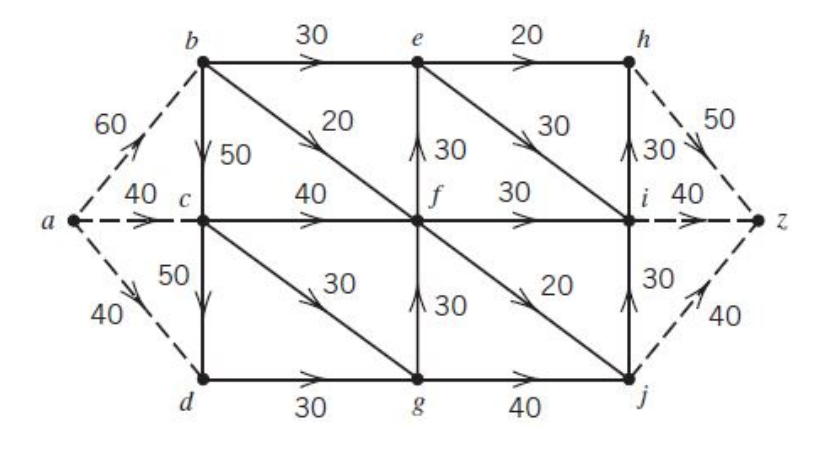
\includegraphics[width=0.5\linewidth]{network_extension-1}
\end{center}

\subsubsection{Šķēlums}
\textbf{Def.}  Šķēlums - šķautņu kopa $E$, ka jebkurš ceļš (a,z) iet caur E.
\textbf{Def.} Šķēluma caurlaidība - \begin{equation}c(E ) = \sum_{uv \in E}{c(uv)}\end{equation} (plūsmas virziens no kopas, kas satur a uz kopu, kas satur z).

Šķēlums ({a, b, c}, {d, e, z}) sastāv no šķautnēm bd, be un ce, bet ne no dc, jo vērsta pretējā virzienā.
%[TK: figure]

\textbf{T. } Plūsma a → z nevar būt lielāka par (Forda-Folkensona algoritms/procedūra, z)-šķēluma caurlaidību

\textbf{T. } Jebkurai a-z plūsmai tīklā plūsma no a ir vienāda ar plūsmu, kas nonāk z.

\textbf{Def.} Plūsmas vērtība |f | ir vienāda ar plūsmu, kas iziet no sākuma virsotnes, jeb saskaņā ar teorēmu plūsmu, kas nonāk z.

\textbf{T. }Jebkurai a-z plūsmai un a-z šķēlumam tīklā |f | ≤ c(E ).

Iepriekšējā teorēma saka, ka a-z plūsmas vērtība nevar pārsniegt jebkura a-z šķēluma caurlaidību. No tā seko, ka kāda a-z plūsma f* ir vienāda ar kādu a-z šķēlumu. Tādā gadījumā f* ir jābūt maksimālās plūsmas lielumam. Pārliecināsimies, ka jebkuram plūsmas tīklam var konstruēt a-z plūsmu, kuras vērtība ir vienāda ar kādu a-z šķēlumu un tā ir plūsma ar maksimālo vērtību.
Intuitīva pieeja, lai risinātu problēmu varētu būt plūsmas sadalīšana pa vienas vienības ceļiem.  Sekojoši maksimālo plūsu varētu veidot skaitot kopā šādus a-z vienas vienības ceļus, vienmēr pārliecinoties, ka nevienas šķautnes caurlaidība nav pārsniegta.  Tādējādi plūsmas papildināšanai varētu izmantot tikai nepiesātinātas šķautnes, tas ir tādas, kur jau uzkonstruētā plūsma neaizņem visu caurlaidību.

Kā izvairīties no šādām situācijām un vai būtu iespējams uzlabot plūsmas ceļu izvēles? Tas ir problemātiski piemērojot iepriekš aplūkoto pieeju, taču ir algoritms/procedūra, kas ļauj uzlabot plūsmu un palielināt plūsmu.  Tīklu ar atrasto plūsmu 7 var pārzīmēt, lai uzskatāmāk redzams, ka caur šķautni bc plūsma virzās pretējāvirzienā ar vērtību 5 (no kopas, kas satur z un kopu, kas satur a).  Par cik vienībām plūsma šķautnē be varētu tapt samazināta?

\subsubsection{Forda-Folkensona algoritms/procedūra}

\textbf{Def.} c'(uv) - šķautnes uv caurlaidība reziduālajā tīklā; Ja nav plūsma u → v vai v → u: c 0 (uv ) = c(uv ); Ja ir plūsma u → v : c 0 (uv ) = c(uv ) − f (uv ); Ja ir plūsma v → u: c 0 (uv ) = c(uv ) + f (uv ); Ja ir plūsma f(uv) un tiek pievienota f'.

Var pārsūtīt plūsmu f 0 ≤ f pretējā virzienā samazinot plūsmu u → v pa f'.

Reziduālais tīkls
%[TK: piemērs]

\section{Sapārojumi grafos}
\subsection{Definīcijas}

\textbf{Def.} Sapārojums ir šķautņu kopa, kur katra virsotne pieder ≤ 1 no šķautnēm. Citiem vārdiem, grafa G sapārojums M (matching) ir G apakšgrafs, kurā nevienai šķautnei nav kopīga virsotne ne ar vienu citu šķautni. Katrai virsotnei sapārojumā ir virsotne 1, tas ir, katra virsotne ir galavirsotne vienai šķautnei. Šķautņu skaits sapārojumā raksturo sapārojuma izmēru |M|.
\textbf{Def.} Maksimāls sapārojums M grafā G ir tad, ja vairs nav iespējams pievienot sapārojumam M papildus citas šķautnes no G.
\textbf{Def.} Sapārojuma maksimums ir tad, ja sapārojumam ir lielākais iespējamais izmērs grafā. Tas ir lielākais maksimālais sapārojums.  Vienam grafam var būt vairāki maksimumi.

\textbf{Def.} Neatkarīgas šķautnes - tām nav kopīgas virsotnes Neatkarīga kopa - satur virsotnes starp kurām nav šķautnes.
\textbf{Def.} Divdaļīgs grafs - virsotnes var sadalīt divās neatkarīgās kopās.
\textbf{Def.} Divdaļīgs grafs ir līdzsvarā, ja tam abās kopās ir vienāds skaits virsotņu.

\subsection{Holla teorēma}

Interesē jautājums - kā atrast sapārojuma maksimumu?  It īpaši interesē, kā atrast pilnu sapārojumu.  Pilns (perfect) sapārojums ietver visas grafa virsotnes un katra virsotne pieder tieši vienai šķautnei.  Katrs pilns sapārojums ir arī maksimāls sapārojums, jo nav iespēja papildus pievienot jaunas šķautnes. Taču maksimuma sapārojums var arī nebūt pilns.  Ja grafam ir pilns sapārojums, tad tam ir pāra skaits virsotņu.

%[TK: piemērs ]

Holla \textbf{T. }Ja pilna sapārojuma nav ⇒ var atrast k virsotnes kreisajā pusē, kas savienotas ar ≤ k − 1 virsotnēm labajā pusē.  Ja ir šāda situācija, tad sapārojuma nav.

\subsection{Pagarinošie ceļi}

Kā konstruēt sapārojumu?  Grafā izvēlas šķautnes saskaņā ar sapārojuma definīciju.  Kā uzlabot šo sapārojumu?

%[TK: piem]

Nepilni pagarinoši ceļi: izvēlas virsotni, kas nav sapārota; veido ceļu pārmaiņus no šķautnēm, kas nepieder sapārojumam (zilas) un šķautnēm, kas pieder sapārojumam (sarkanas); ceļu noslēdz ar virsotni, kas ir sapātota, izvēlas virsotni, kas nav sapārota; apluko virsotnes, kur no tās var nokļūt pa nepilnu pagarinošu ceļu; ja nav pagarinoša ceļa, tad esošo sapārojumu nevar palielināt.

\textbf{T. } Ja sapārojums M nav maksimāls, tad esksitē pagarinošs ceļš.

\subsection{Plūsmas tīklā metode}

Plūsmas grafa izmantošana, lai risinātu divdaļīga grafa sapārošanas uzdevumu. Dotam divdaļu grafam G = (A u B, E ) orientē šķautnes no A uz B, pievieno jaunas virsotnes: sākuma virsotni a un beigu virsotni z. Pievieno papildus orientētas šķautnes no a uz katru virsotni A. Pievieno papildus orientētas šķautnes no virsotnēm B uz beigu virsotni z. Visas šķautņu caurlaides spējas pieņem kā 1. Atrisina maksimālās plūsmas problēmu jaunizveidotajā grafā G'.  Šķautnes, kas tiek izmantotas maksimālās plūsmas tīklā atbilsts maksimuma sapārojumam.

\textbf{Def.}  Grafs ir sakarīgs, ja jebkurām virsotnēm u, v eksistē ceļš no u uz v.

\section{Sakarīgs un nesakarīgs grafs}

\textbf{Def.}  Grafa sakarīgā komponente G'=(V',E'), kur V' ir maksimālā virsotņu kopa ar īpašību,
ka katrām divām virsotnēm u,v ∈ V 0 eksistē ceļš u → v , E':uv ∈ E , u ∈ V 0 , v ∈ V 0 .

\subsection{Sakarīga komponente}

\textbf{Def.}  Par grafa G sakarīgo komponenti jeb komponenti sauc jebkuru maksimālu sakarīgu apakšgrafu.  Maksimāls nozīmē, ka apakšgrafam zūd sakarības īpašība, ja tam pievieno vēl kādu no grafa G virsotnēm. Tas nozīmē, ja apakšgrafu var papildināt līdz lielākam, bet tomēr vēl sakarīgam, tad vēl nav bijusi aplūkota komponente.  Sakarīgu komponenšu skaitu apzīmē ar s.  Grafu G sauc apr viensakarīgu, ja tas ir sakarīgs, bet atmetot vienu virsotni v līdz ar tai incidentām šķautnēm, rodas nesakarīgs grafs. Šādu virsotni v sauc par sasaistes virsotni.

\textbf{Def.} Grafu G sauc par divaskarīgu, ja tas nav viensakarīgs, bet atmetot 2 virsotnes vi un vj un tām incidentās šķautnes - rodas nesakarīgs grafs. Trīssakarīgs ir tāds grafs, kas nav divsakarīgs, bet atmetot 3 virsotnes ar tām incidentām šķautnēm, rodas nesakarīgs grafs.

k-sakarība
\textbf{Def.} Ceļa iekšējās virsotnes - virsotnes, kas nav tā gali.  Grafs ir k-sakarīgs, ja katrām tā divām virsotnēm eksistē vismaz k šīs virsotnes savienojošu ceļu bez kopējām iekšējām virsotnēm (iekšēji nešķeļošies ceļi).  Visiem k1 > k2 no k1-sakarības seko k2-sakarība.  Par grafa sakarības skaitli, sauc lielāko k, pie kura šis grafs ir k-sakarīgs.

Koks ir 1-sakarīgs, bet nav 2-sakarīgs.  Ja grafs ir nesakarīgs, tad tas ir 0-sakarīgs un nav 1-sakarīgs.  Grafs ir sakarīgs, tad un tikai tad, ja tas ir 1-sakarīgs.  Pilns grafs Kn ir (n – 1)-sakarīgs.  Ja grafs ir k-sakarīgs, tad k ≤ mind(v), kur d(v) ir virsotnes v pakāpe.

\subsubsection{Sadalošā un atdalošā kopa}

\textbf{Def.}  Sakarīga grafa G = (V, E) virsotņu apakškopu S sauc par sadalošo kopu, ja grafs
G(V—S) ir nesakarīgs.
Sakarīga grafa sadalošā virsotne veido sadalošo kopu.  Grafam Kn nav nevienas sadalošās kopas.

\textbf{Def.}  Grafa G = (V, E) virsotņu apakškopu S sauc par virsotnes x un y atdalošo kopu, ja x un y pieder dažādām G(V – S) sakarīgajām komponentēm.

\textbf{Def.} Šķēlums ir šķautņu kopa, kuru izmetot grafs sadalās divās daļās.

\subsection{Teorēmas}

\subsubsection{Mengera teorēma}
Kāds ir mazākais šķautņu skaits šķēlumā, kas atdala A no B?
Mengera \textbf{T. } Ja mazākajā šķēlumā, kas atdala A no B ir k šķautnes, tad var atrast k ceļus no A uz B, kuriem nav kopīgu šķautņu.  (Min šķēlums) = (Max ceļu skaits no A uz B bez kopīgām virsotnēm). Lielākais iespējamais nekaimiņu virsotnes x un y savienojošu iekšēji nešķeļošos ceļu skaits vienāds ar mazākās x un y atdalošās kopas apjomu.

\subsection{Forda-Folkensona T.}
\textbf{T. }(Max plūsma A → B) = (Min šķēlums, kas atdala A un B)
Apgalvojums: (Max ceļu skaits bez kopīgām virsotnēm) = (Max plūsma)

\printindex

\end{document}